\documentclass[a4paper,12pt, projekat]{etf}

\usepackage[intlimits]{amsmath}
\usepackage{amsmath, amsfonts, amssymb, graphicx}

\usepackage[serbian]{babel}
\usepackage[T1]{fontenc}
\usepackage[utf8]{inputenc}
\usepackage{graphicx}

\addto\captionsserbian{\renewcommand{\bibname}{Literatura}}

\title{Poredjenje vremena filtriranja na STM32F4 mikrokontroleru i PC-u}
\author{Lazar Caković}
\indeks{3083/2016}
\date{jul 2018.}
\mentor{prof.~dr Nenad Jovi\v{c}i\'{c}}
\predmet{32bitni mikrokontroleri}

\begin{document}

\maketitle

\tableofcontents

\listoffigures

\newpage

\chapter{Uvod}
Cilj projekta iz predmeta 32-bitni mikrokontroleri, na master studijama odseka
za Elektroniku, bio je da se uporedi filtriranje signala u vremenskom i frekvencijskom
domenu na mikrokontroleru STM32F407VG i PC-u kori\v{s}\'{c}enjem MATLAB programskog paketa.
Poredjenje filtriranja se vr\v{s}ilo na brzinu izvr\v{s}avanja filtriranja, kao i na
odstupanje signala dobijenog filtriranjem na mikrokontroleru od onog dobijenog u programskom
paketu MATLAB. Projekat je radjen u softverskim paketima MATLAB i IAR Embedded Workbench for ARM,
a na plo\v{c}i STM32F4 Discovery.

\newpage

\chapter{Opis sistema}
U implementaciji projekta, sistem je konfigurisan tako da se deo projekta izvr\v{s}ava na PC-u,
u okviru MATLAB programskog paketa. Dok se drugi deo izvr\v{s}ava na samoj razvojnoj plo\v{c}i.
Na PC-u je izgenerisan signal koji je potrebno obraditi. Razvojna plo\v{c}a Discovery je povezana
na PC, i kori\v{s}\'{c}enjem \textit{semihosting-a} implementirana je emulacija \textit{file system-a}
tako da je omogu\'{c}eno \v{c}itanje i upis u fajlove PC-a.

\newpage

\chapter{Softverska implementacija}
Kao \v{s}to je ve\'{c} navedeno, softverska implementacija je izvr\v{s}ena na PC-u, u okviru MATLAB
programskog paketa, i na strani mikrokontrolera u okviru IAR razvojnog okru\v{z}enja. Pa \'{c}e tim
redom i biti opisane.

\section{MATLAB implementacija}
U ovom delu softverske implementacije, izgenerisan je signal kao zbir dve sinusoide razli\v{c}itih
frekvencija koji je potrebno izfiltrirati. Konkretno, kao primer, uzet je zbir dve sinusoide od 2KHz
i 10KHz, sa frekvencijom odabiranja od 50KHz, u 256 ta\v{c}aka. Ovaj broj ta\v{c}aka je uzet zbog
ograni\v{c}enja razvojne plo\v{c}e koja se koristi u drugom delu implementacije, po\v{s}to se ovde
izgenerisan signal koristi u daljoj implementaciji. Takodje, u ovom delu se generi\v{s}u i odbirci
filtra koji \'{c}e biti kori\v{s}\'{c}en u filtriranju kako u ovom delu, tako i u drugom delu
implementacije. Filtar koji se koristi je filtar propusnik niskih u\v{c}estanosti, 120og reda, sa
grani\v{c}nom u\v{c}estanosti od 8kHz, i slabljenjem u propusnom opsegu od 0.01dB i u nepropusnom
opsegu od 80dB. Za dobijanje odbiraka filtra koristi se ugradjena funkcija u MATLAB-u \textbf{fircegrip}.

\begin{table}[h!]
	\begin{tabular}{lll}
		\includegraphics[scale=0.4]{matlab_raw.png} &
		\includegraphics[scale=0.4]{matlab_raw_spec.png} \\
		MATLAB: Ulazni signal &
		MATLAB: Spektar ulaznog signala
	\end{tabular}
\end{table}

\begin{figure}[htb]
	\centering
	\includegraphics[scale=0.3]{matlab_filter.png}
	\caption{MATLAB: Karakteristika filtra}
	\label{fig:matlabFilter}
\end{figure}

Filtriranje signala u MATLAB-u se vr\v{s}i u vremenskom i frekvencijskom domenu. Filtriranje signala
u frekvencijskom domenu se vr\v{s}i kori\v{s}\'{c}enjem ugradjene funkcije \textit{filter}, uz pomo\'{c}
koje se dobija isfiltriran signal kao na slici ispod. Filtriranje u frekvencijskom domenu vr\v{s}i
se mno\v{z}enjem FFT predstave signala i filtra. Nakon \v{c}ega se dobija isti rezultat kao u
prethodnoj implementaciji.

\begin{table}[h!]
	\begin{tabular}{ll}
		\includegraphics[scale=0.4]{matlab_filtered.png} &
		\includegraphics[scale=0.4]{matlab_filtered_fft.png} \\
		MATLAB: Izlazni signal (FIR) &
		MATLAB: Spektar izlaznog signala (FIR)
	\end{tabular}
\end{table}


\begin{table}[h!]
	\begin{tabular}{ll}
		\includegraphics[scale=0.4]{matlab_fft_filter.png} &
		\includegraphics[scale=0.4]{matlab_fft_filtered.png} \\
		MATLAB: Izlazni signal (FFT) &
		MATLAB: Spektar izlaznog signala (FFT)
	\end{tabular}
\end{table}

Kao \v{s}to je navedeno, odbirci signala koji su generisani, upisuju se u binarne fajlove koji \'{c}edef
se koristiti u implementaciji na mikrokontroleru. Ispod je prikazano vreme izvr\v{s}avanja delova koda u
programskom paketu MATLAB.

\begin{figure}[htb]
	\centering
	\includegraphics[scale=0.8]{matlab_times.png}
	\caption{MATLAB: Vremena izvr\v{s}avanja filtriranja u sekundama}
	\label{fig:matlabTimes}
\end{figure}

\section{Implementacija na mikrokontroleru}
U ovom delu softverske implementacije, filtriranje ve\'{c} izgenerisanih signala se vr\v{s}i na
strani mikrokontrolera. Ova implementacija je izvr\v{s}ena u IAR Embedded Workbench for ARM razvojnom
okru\v{z}enju koji sadr\v{z}i IAR kompajler za ARM arhitekture.

Kako su odbirci signala koji je potrebno izfiltrirati, kao i odbirci filtra koji se koristi za filtriranje
sme\v{s}teni u binarne fajlove, na strani mikrokontrolera kori\v{s}en je mehanizam \textit{semihosting-a}.
\textit{Semihosting} je mehanizam koji omogu\'{c}ava kodu koji se pokre\'{c}e na ARM platfomi da komunicira
i koristi ulazno-izlazne mehanizme na \textbf{host} PC-u, odnosno na PC-u na kome se pokre\'{c}e razvojno
okru\v{z}enje. Ovaj mehanizam omogu\'{c}ava sve operacije sa fajlovima na ARM mikrokontroleru, kao i ispis
i \v{c}itanje u Debug terminalu unutar razvojnog okru\v{z}enja. Kori\v{s}enjem ovog mehanizma, pojednostavljen
je pristup podacima koji se nalaze na samom PC-u, ali ovaj mehanizam ima ograni\v{c}enje, a to je da se mo\v{z}e
koristiti samo u delu projektovanja i debug-ovanja sistema. Odnosno, samo ukoliko se debugger koristi. Ukoliko
se \v{z}eli posti\'{c}i da sistem radi samostalno, potrebno je na\'{c}i novi na\v{c}in za dobijanje podataka na
mikrokontroleru, bilo to prenosom preko serijskog interfejsa, ili na neki drugi na\v{c}in.
Nakon dobijanja svih potrebnih podataka na mikrokontroleru, implementirana su dva na\v{c}ina filtriranja, kao i
u prethodnom delu. A to je filtriranje u vremenskom i frekvencijskom domenu. Oba na\v{c}ina filtriranja su
implementirana kori\v{s}\'{c}enjem CMSIS bibilioteke i njenih fukncija za \textbf{fir} filtriranje, kao i
funkcija za \textbf{fft}.

Za filtriranje u vremenskom domenu, kori\v{s}\'{c}ena je funkcija \textbf{arm\_fir\_f32} koja vr\v{s}i filtriranje
signala \textbf{fir} filtrom. Funkcija za filtriranje se izvrsava nad blokovima velicine 16 podataka, i formira
izlazni signal. Nakon \v{c}ega se izfiltriran signal sme\v{s}ta u izlazni binarni fajl. Nakon \v{c}ega se mo\v{z}e
porediti u MATLAB-u.

Takodje, filtiranje u frekvencijskom domenu se vr\v{s}i kori\v{s}\'{c}enjem funkcija iz CMSIS biblioteke, i to
konkretno funkcije \textbf{arm\_cfft\_f32}, kojom se dobija FFT ulaznog signala i filtra. Nakon \v{c}ega se vr\v{s}i
mno\v{z}enje FFT predstava signala i filtra u kompleksnom domenu. I na posletku, istom funkcijom \textbf{arm\_cfft\_f32}
se radi inverzna FFT. Kao i u prethodnom delu, izlazni signal se sme\v{s}ta u binarni fajl, nakon \v{c}ega se mo\v{z}e
porediti u MATLAB-u.

\begin{table}[h!]
	\begin{tabular}{ll}
		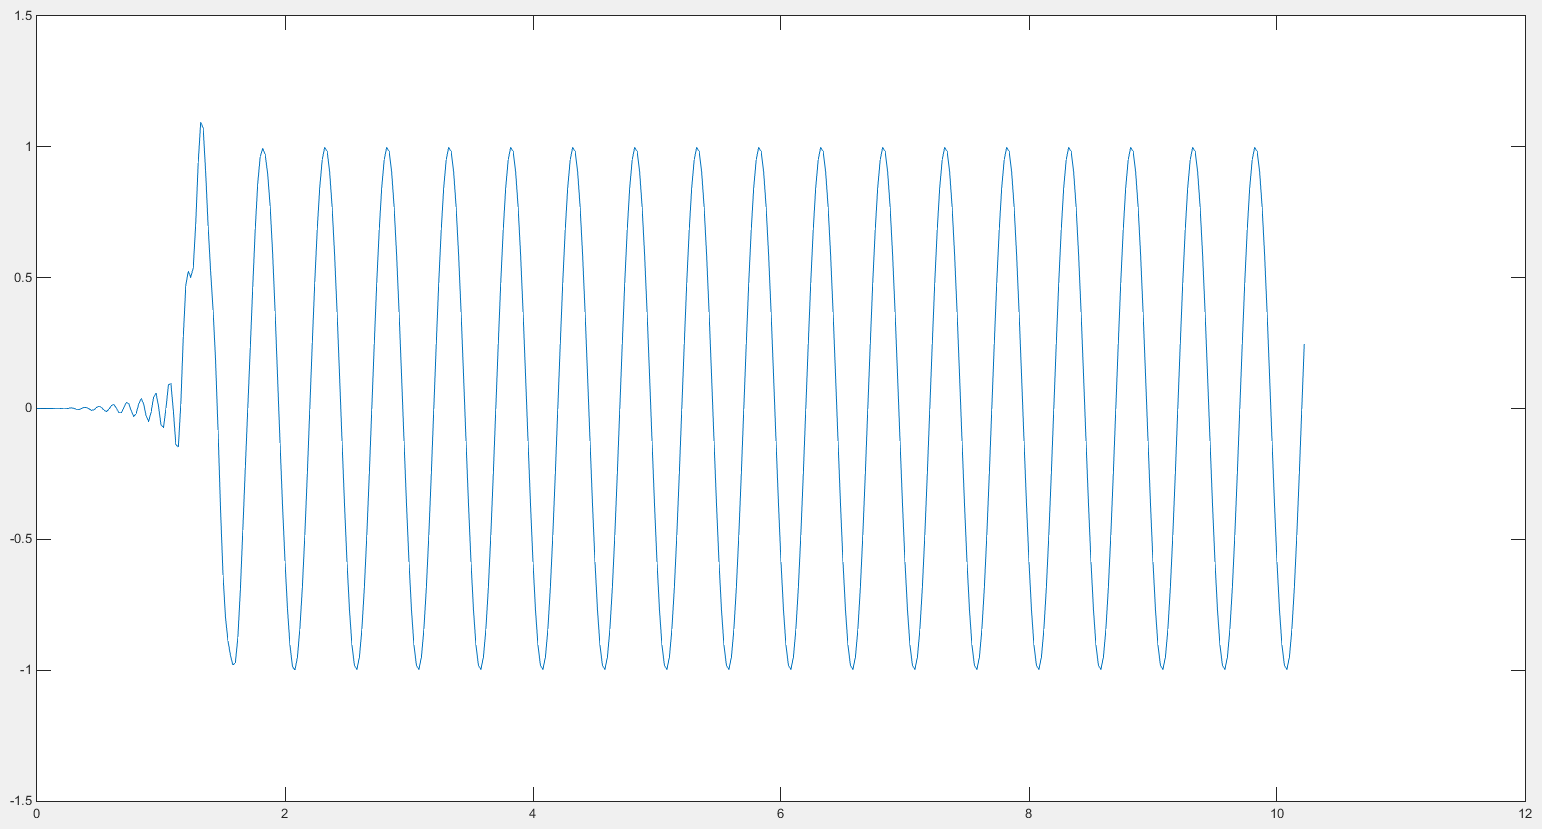
\includegraphics[scale=0.16]{mcu_fir_signal.png} &
		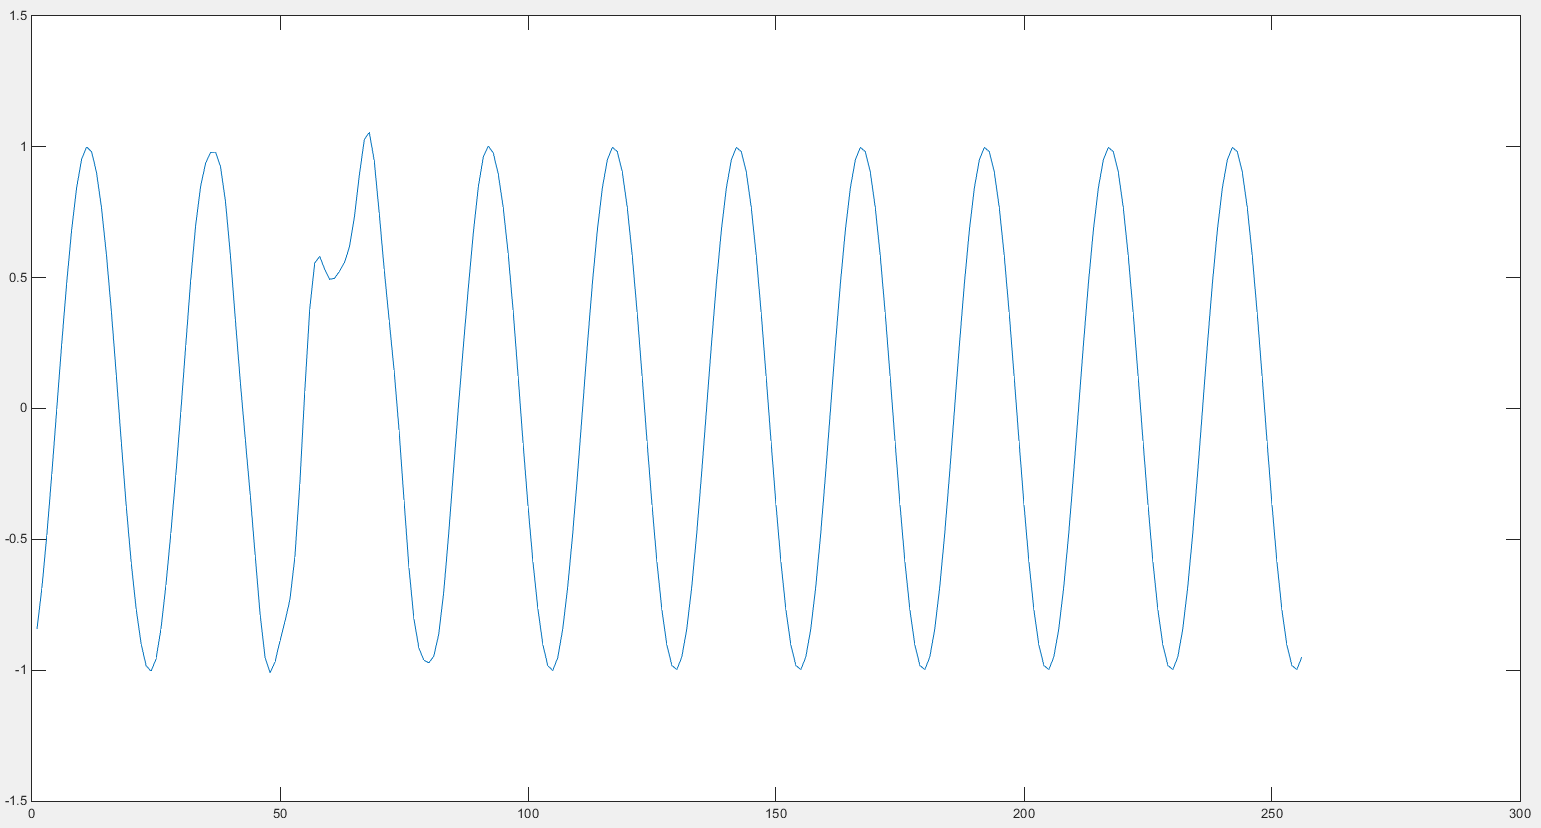
\includegraphics[scale=0.16]{mcu_fft_signal.png} \\
		MCU: Izlazni signal (FIR) &
		MCU: Izlazni signal (FFT)
	\end{tabular}
\end{table}

Ispod je prikazano vreme izvr\v{s}avanja delova koda na strani mikrokontrolera.

\begin{table}[h!]
	\begin{tabular}{ll}
		\includegraphics[scale=0.5]{mcu_fir_time.png} &
		\includegraphics[scale=0.5]{mcu_fft_time.png} \\
		MCU: Vreme filtriranja (FIR) &
		MCU: Vreme filtriranja (FFT)
	\end{tabular}
\end{table}

\chapter{Poredjenje rezultata}

Rezultati dobijeni na PC-u i mikrokontroleru su isti. Tj. rezultat filtriranja ulaznog signala je isti.
Kori\v{s}\'{c}enjem datih signala, dobija se identi\v{c}an rezultat na kraju filtriranjem u vremenskom i
u frekvencijskom domenu. Takodje, treba uzeti u obzir i vremena izvr\v{s}avanja. Uvidja se da je filtriranje
u frekvencijskom domenu u programskom paketu MATLAB sporije nego filtriranje u vremenskom domenu. To se mo\v{z}e
objasniti optimizacijom funkcija koje su kori\v{s}\'{c}ene za vremensko filtriranje.
Vremena izvr\v{s}avanja na mikrokontroleru su druga\v{c}ija od vremena u MATLAB-u, i vidi se da je izvr\v{s}avanje
filtriranja u vremenskom domenu dva puta sporije od filtriranja u frekvencijskom domenu, gde treba uzeti u obzir da
podataka koji se filtriraju u frekvencijskom domenu ima dva puta manje, zbog ograni\v{c}enja razvojne plo\v{c}e.
Takodje, i u ovom slu\v{c}aju je kori\v{s}\'{c}ena specijalizovana biblioteka za obradu signala, CMSIS DSP.
Iz ovoga se mo\v{z}e zalju\v{c}iti da kori\v{s}\'{c}enje funkcija za filtriranje odredjuje u mnogome brzinu sistema.


\end{document}
